\documentclass[10pt, scrartlc]{article}
%\documentclass{article}
\usepackage[font={sf}]{caption}
\usepackage[]{graphics}
\usepackage{graphicx}
\usepackage{epstopdf}
\usepackage{hyperref}
\hypersetup{breaklinks=true, colorlinks=true, citecolor=blue}
\usepackage{natbib}
\usepackage{color}
\usepackage{soul}
\usepackage{rotating}
\usepackage{tabularx}
\usepackage{longtable}
\usepackage{lscape}
\usepackage{array}
\usepackage{multirow}
\usepackage{setspace}
\usepackage{textcomp}
\usepackage{dcolumn}
\setlength{\LTcapwidth}{6in}
\usepackage{dcolumn}
\usepackage[margin=1in]{geometry}
\usepackage{tocloft}
\usepackage{caption}

 \bibpunct{(}{)}{,}{a}{}{,}
 \doublespacing
 \raggedright
 \setlength{\parindent}{15pt} 


\begin{document}

\pagecolor{white}

\begin{center}
{ \Large \bf Figures }
\end{center}

\listoffigures

\clearpage
\newpage

\begin{figure}[h]
	\begin{center}
		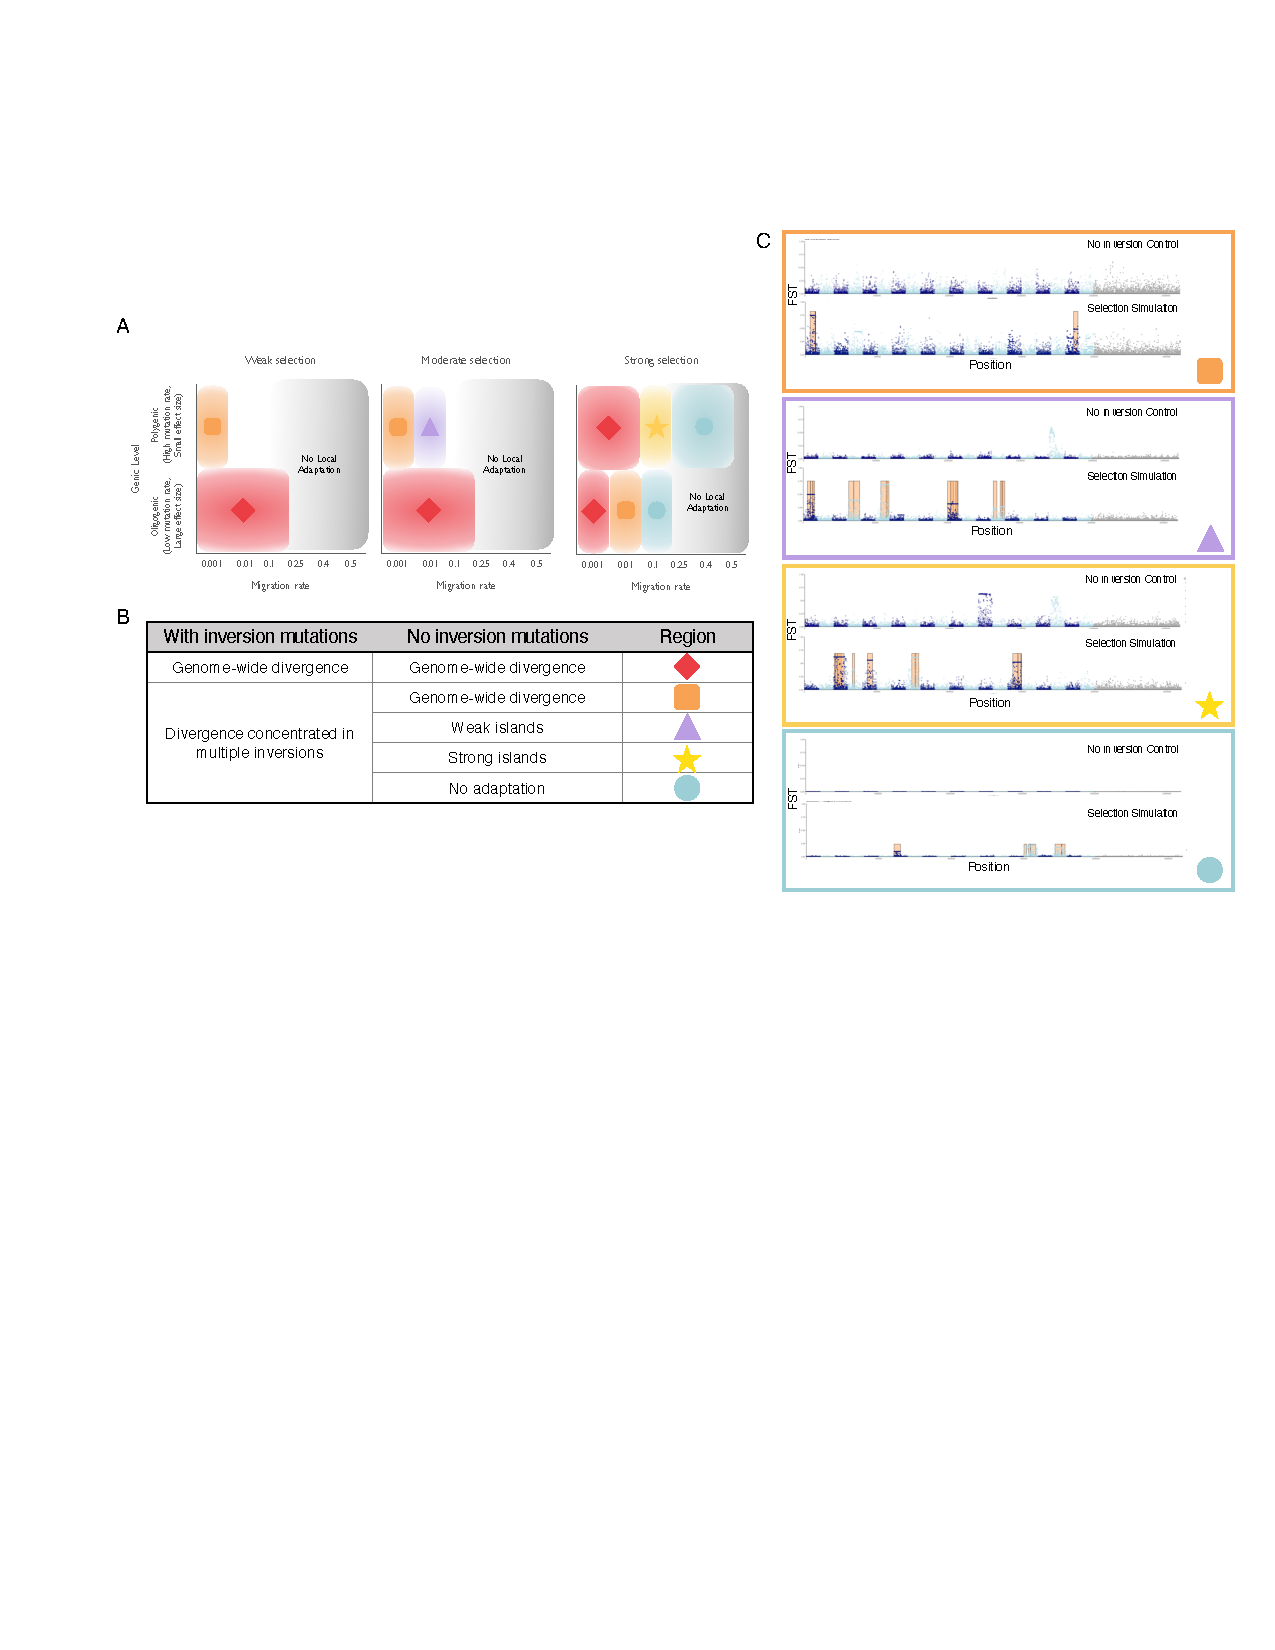
\includegraphics[width = 6.5in]{Fig1_ConceptFig.pdf}
	\end{center}
	\caption[Genomic Basis of Local Adaptation Regions]{Description of five conceptual regions that correspond to different genomic architectures that underlie trait divergence across our parameter space (A-B). Each region corresponds to what occurred in both with-inversion simulations (B with-inversion mutation column) and paired no-inversion control simulations (B no-inversion mutation column). Manhattan plot examples are provided for four regions with no-inversion example on top and with-inversion on the bottom (C). Alternating light and dark blue represent different chromosomes and yellow bars represent inversions present in the population. }
\end{figure}

\clearpage
\newpage

\begin{figure}[h]
	\begin{center}
		\includegraphics[width = 6.5 in]{Fig2_LA.pdf}
	\end{center}
	\caption[Local Adaptation]{The average amount of local adaptation that is reached in simulations that include inversions plotted as a function of migration rate and split between three panels representing weak, moderate and strong selection for the A) oligogenic and B) polygenic architectures. The ribbon represents one standard deviation for the average local adaptation expected under the null which is the paired no-inversion control simulations. The difference between the average local adaptation reached in with-inversion simulations and paired no-inversion control simulation is shown for the C) oligogenic and D) polygenic architectures. The percent of additive genetic variance found inside inverted regions is plotted for the E) oligogenic and F) polygenic architectures. The ribbon represents one standard deviation for the average percent of the genome that is inverted. The average number of adaptive inversions is plotted for the G) oligogenic and H) polygenic architectures. All averages are across five replicate simulations and all error bars represent one standard deviation.}
\end{figure}

\clearpage
\newpage

\begin{figure}[h]
	\begin{center}
		\includegraphics[width = 6.5 in]{Fig3_characteristics.pdf}
	\end{center}
	\caption[Inversion Characteristics]{The average of three inversion characteristics across five replicate simulations is plotted as a function of migration rate and split between three panels representing weak, moderate and strong selection for adaptive inversions in orange, nonadaptive inversions in light grey, and inversions from the no-selection control simulation in black. Inversion age in generations (gen) is plotted for a A) polygenic architecture and B) oligogenic architecture. Average inversion length in base pairs (bp) is plotted for a C) polygenic architecture and D) oligogenic architecture. Average number of inversion quantitative trait nucleotides (QTNs) scaled by the total length of the inversion plotted for a E) polygenic architecture and F) oligogenic architecture. Blank spaces represent those parameter combinations where no adaptive inversions evolved. Region symbols for simulations with local adaptation are plotted at the bottom of the figure. }
\end{figure}

\clearpage
\newpage


\begin{figure}[h]
	\begin{center}
		\includegraphics[width = 6.5 in]{Fig4_evoHist.pdf}
	\end{center}
	\caption[Evolutionary History of Adaptive Inversions]{The average number of adaptive inversions (across five replicate simulations) is plotted for our three possible categories: capture then gain (light green), capture then no gain (blue green), and neutral then gain (purple). The plots are plotted for the A) polygenic and B) oligogenic architectures with data split for migration rate on the x-axis and selection strength as the three panels within each plot. Region symbols for simulations with local adaptation are plotted at the bottom of the figure. C) The sum of inversion effect size on the phenotype is plotted through time for one simulation where inversions facilitated adaptation for adaptive inversions (left panel), nonadaptive inversions (middle panel) and no selection simulations (right panel). Colors represent which population the inversion was diverging in and the size of points through time was the FST value for that inversion at each time step.}
\end{figure}


\end{document}